\documentclass{article}
\usepackage[utf8]{inputenc}
% make subsections alphabetic:
\renewcommand{\thesubsection}{\thesection.\alph{subsection}}

% vector drawing package
\usepackage{tikz}

% reals set symbols
\usepackage{amssymb}

\title{Intro to Linear Algebra: Workshop 1}

\date{May 2020}

\begin{document}

\maketitle

\section{}
Observe that $v = (0.5, 0.5, 0), u = (0.9, 0.1, 0) \in S$, 
\newline 
but $v + u = (1.4, 0.6, 0) \notin S$
\newline
\newline
Similarly, for scalar $s = 10$ and $v = (0.5, 0.5, 0)$, $s.v = (5, 5, 0) \notin S$
\section{}
For positive integer n, define $+$ and $.$ as follows:\newline

$$\forall 
u=\left[\begin{array}{c}u_0 \\.\\.\\.\\u_n\end{array}\right],
\forall
v=\left[\begin{array}{c}v_0 \\.\\.\\.\\v_n\end{array}\right]
\in \mathbb{R}^2, u + v = \left[\begin{array}{c}u_0 + v_0\\.\\.\\.\\u_n + v_n\end{array}\right]$$ 

$$\forall 
u=\left[\begin{array}{c}u_0 \\.\\.\\.\\u_n\end{array}\right]\in \mathbb{R}^2,
\forall
s \in \mathbb{R}, 
s . u = \left[\begin{array}{c}s u_0\\.\\.\\.\\s u_n\end{array}\right]$$
It is easy to see due to properties of $\mathbb{R}$, for any positive integer n and $u, v\in \mathbb{R}$, this:\newline
Is commutative: $u_n + v_n = v_n + u_n$.\newline
Is associative: for any $w \in \mathbb{R}$, $(u_n + v_n) + w_n = u_n + (v_n + w_n)$ and $u_n (v_n w_n) = (u_n v_n) w_n$.\newline
Has additive identity: $u + 0 = u$ for vector $0=\left[\begin{array}{c}0\\.\\.\\.\\0\end{array}\right]$ since $u_n + 0 = u_n$.\newline
Has additive inverse: $u + x = 0$ for vector $x = \left[\begin{array}{c}-u_0\\.\\.\\.\\-u_n\end{array}\right]$ since $u_n + (-u_n) = 0$.\newline
Is distributive: for scalar s and d, $s(u_n+v_n) = s u_n + s v_n$ then $s . (u + v) = s . u + s . v$. Also, $(s+d) u_0 = s u_0 + d u_0$ then $(s + d) . u = s . u + d . u$.\newline
Conforms to unitary law: $1 . v = v$ since $1 v_n = v_n$.\newline
\newline
Addition:\newline
for $u = (5, 0), v = (5, 2)$\newline
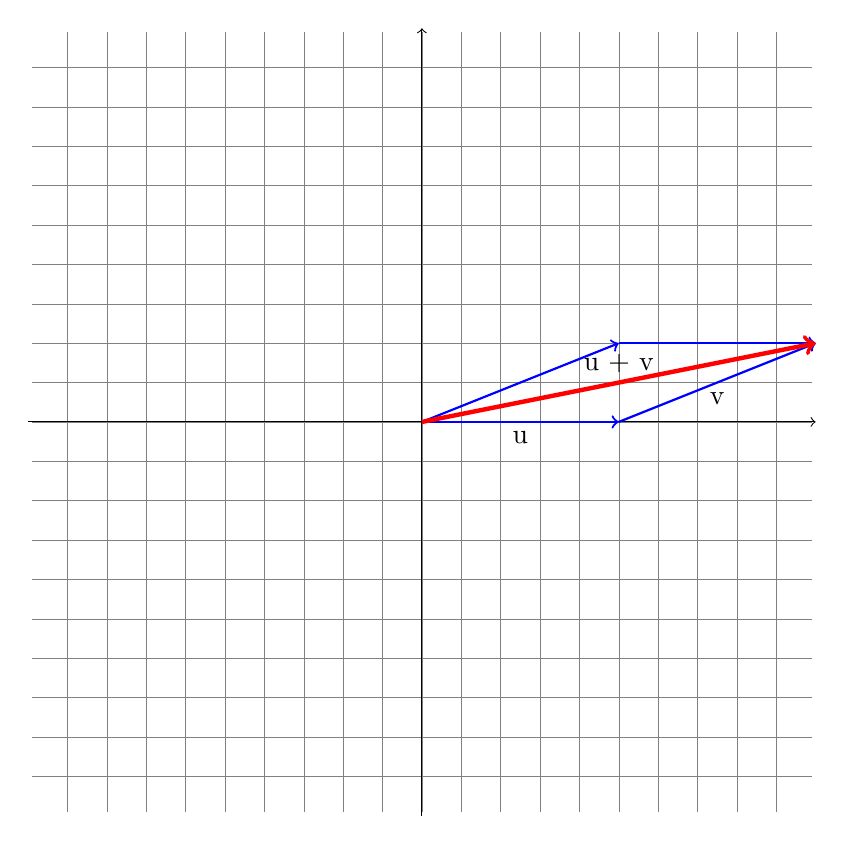
\begin{tikzpicture}[scale=0.5]
\draw[very thin,color=gray] (-9.9,-9.9) grid (9.9,9.9);
\draw  [->] (0,-10) -- (0,10);
\draw  [->] (-10,0) -- (10,0);
\draw [->, thick, blue] (0,0) -- (5,0);
\draw [->, thick, blue] (5,2) -- (10,2);
\draw [->, thick, blue] (5,0) -- (10, 2);
\draw [->, thick, blue] (0,0) -- (5, 2);
\draw [->, ultra thick, red] (0,0) -- (10, 2);
\node [below] at (2.5, 0) {u};
\node [below] at (7.5, 1) {v};
\node [above] at (5,1) {u + v};
\end{tikzpicture}\newline
Scalar multiplication:\newline
for $u = (1, 3), s = 3$\newline
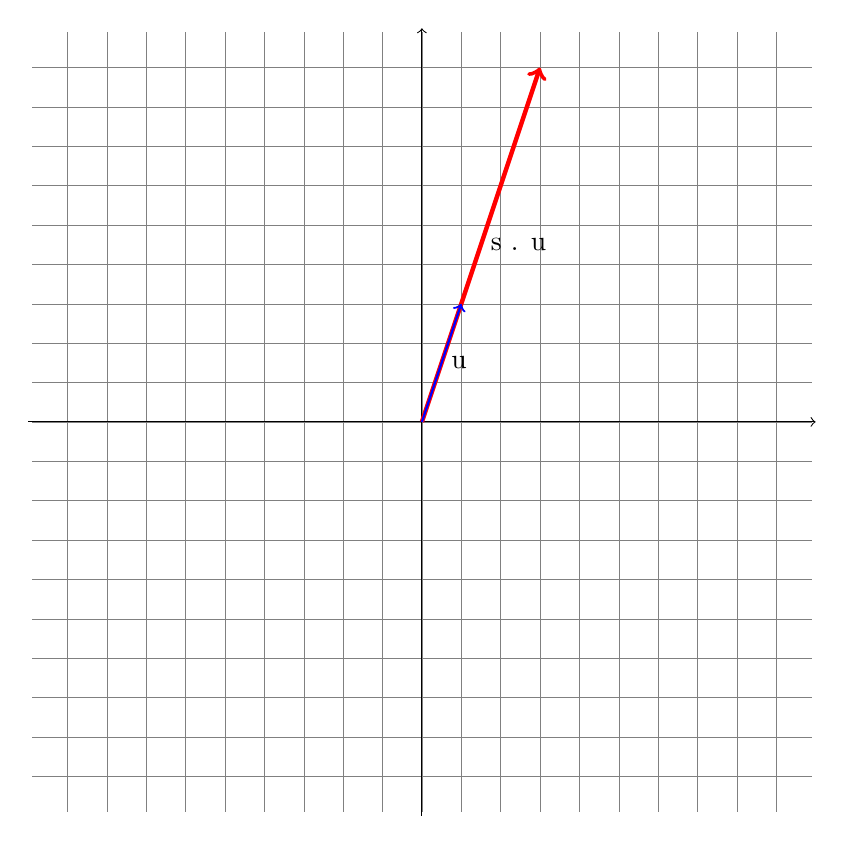
\begin{tikzpicture}[scale=0.5]
\draw[very thin,color=gray] (-9.9,-9.9) grid (9.9,9.9);
\draw  [->] (0,-10) -- (0,10);
\draw  [->] (-10,0) -- (10,0);
\draw [->, ultra thick, red] (0,0) -- (3, 9);
\draw [->, thick, blue] (0,0) -- (1,3);
\node [right] at (0.5, 1.5) {u};
\node [right] at (1.5,4.5) {s . u};
\end{tikzpicture}
\end{document}
